\chapter{Background and Theory}
% This chapter should describe the theoretical background needed to understand
% and solve the problem. For instance, a description of the hardware platform
% or specific components involved in this assignment, definition of concepts
% that are important to understand the solution should be summarized here. Add
% citations to show sources whenever appropriate.

This chapter gives a brief introduction to the EFM32GG-DK3750 and various hardware components that were involved in the exercise. In addition, it will also introduce some concepts and underlying theory.

\section{Overview of EFM32GG-DK3750}
Through the exercises in this course we will work with the Silicon labs EFM32GG-DK3750 prototyping board (figure \ref{fig:efm-board}), from here on referenced as EFM32GG. The EFM32GG have several hardware components and on-board peripherals that are of special interest for this exercise:
\begin{itemize}
	\item General-Purpose Input/Output pins
	\item Gamepad Prototype
	\item Clock Management Unit
	\item Energy Management Unit
	\item Direct Memory Access controller
	\item Digital to Analog Converter
  % TODO: Add the components used in exercise 2 to this list
\end{itemize}
This chapter will give an introduction to each of those devices, and will highlight the relevant features. For a map of the EFM32GG hardware components, see figure \ref{fig:giant-gecko-map}.

\begin{figure}[ht]
  \centering
  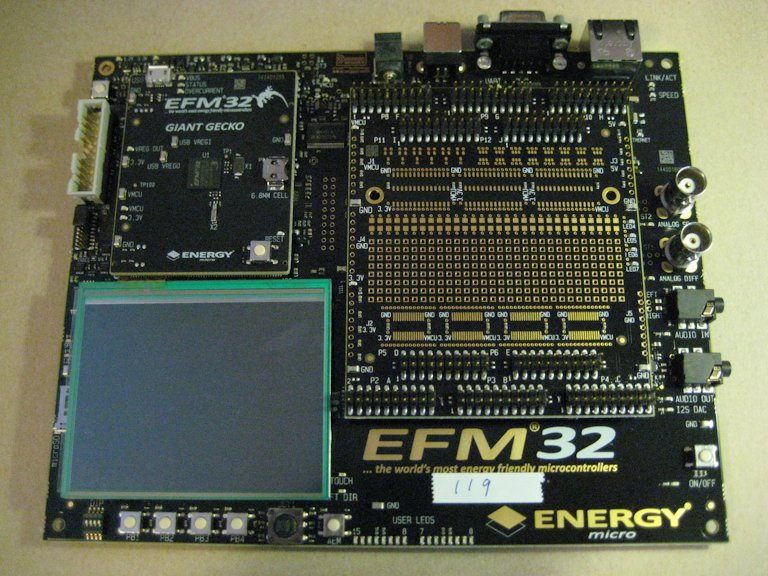
\includegraphics[width=0.7\textwidth]{images/efm_board.jpg}
  \caption{The EFM32GG prototyping board}\label{fig:efm-board}
\end{figure}

\begin{figure}[ht]
  \centering
  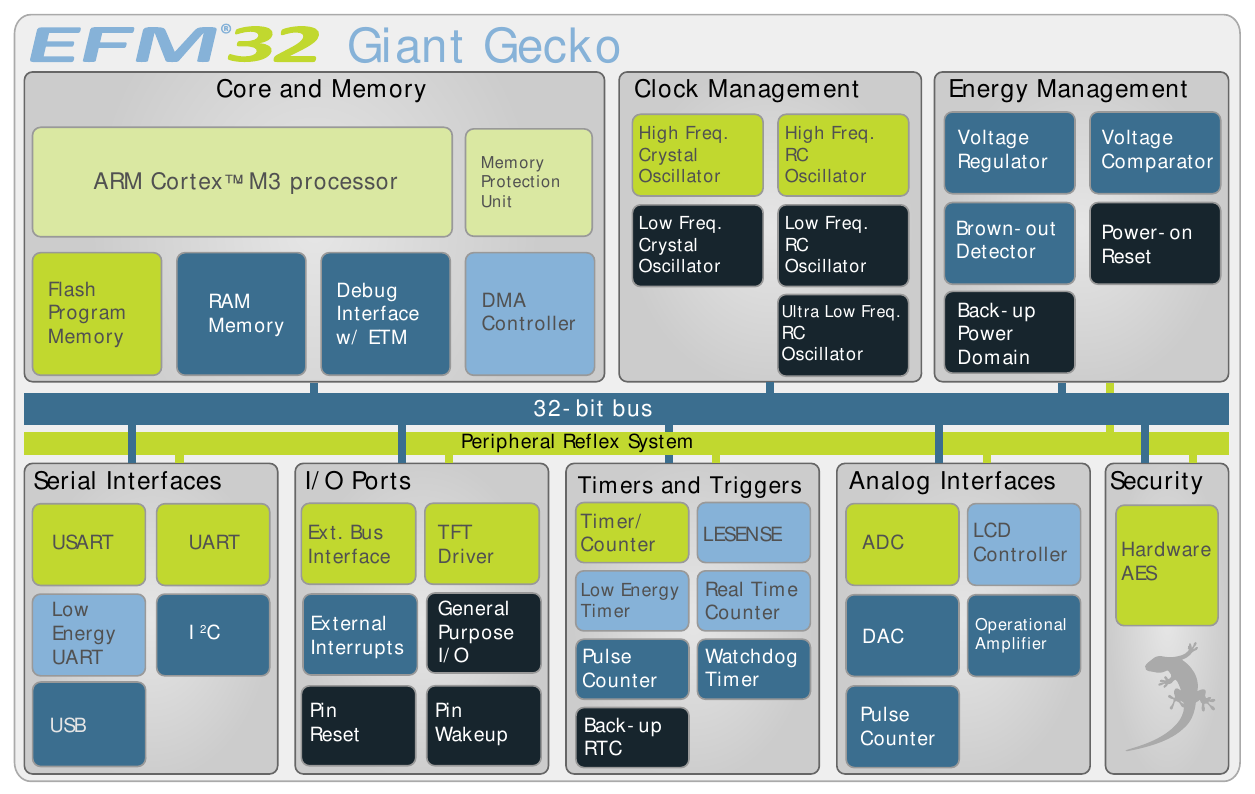
\includegraphics[width=\textwidth]{images/giant_gecko_map.png}
  \caption{Map of the EFM32GG hardware components}\label{fig:giant-gecko-map}
\end{figure}


\section{Clock Management Unit}\label{sec:cmu}
The Clock Management Unit (CMU) controls the on-board oscillators and clocks, and produces clock signals that drives the core modules and all the peripherals. The CMU can enable or disable clock signals for the peripherals on an individual basis, and the power consumption is reduced significantly by only enabling the clock for the peripherals that will be used. By default, the clock for all peripherals is disabled. 

The CMU manages several system clocks in order to provide different clock signals to the core modules and the peripherals. These system clocks include the High Frequency Clock (HFCLK), the High Frequency Core Clock (HFCORECLK), and the High Frequency Peripheral Clock (HFPERCLK).\cite{efm32gg-rm}

\subsection{High Frequency Clock}
HFCLK drives two prescalers that generate HFCORECLK and HFPERCLK, in addition to driving the CMU itself. With separate prescalers it is possible to configure the clock speeds of the core modules and the peripherals individually. The HFCLK itself can be driven either by one of the high-frequency oscillators (HFRCO and HFXO), or by one of the low-frequency oscillators (LFRCO and LFXO). 

\subsection{High Frequency Core Clock}
HFCORECLK is the clock that drives the core modules, which consists of the CPU and tightly coupled modules such as the DMA. The frequency of HFCORECLK can be changed dynamically by writing to CMU\_HFCORECLKDIV, and the clock can be disabled for individual modules by clearing bits in CMU\_HFCORECLKEN0. 

\subsection{High Frequency Peripheral Clock}
HFPERCLK is the clock that drives the high-frequency peripherals. The frequency of the HFPERCLK can be changed dynamically by writing to CMU\_HFPERCLKDIV, and the clock can be disabled for individual peripherals by clearing bits in CMU\_HFPERCLKEN0. 

%TODO: Write about other clocks

\subsection{Oscilliators}
TODO % TODO: Write about oscilliators


\section{TIMER (Timer/Counter)}
The TIMER module can be used to count events and trigger actions in other peripherals without involving the CPU. It can also be used to trigger interrupts after a specific time interval. It has a 16 bit counter that is either incremented or decremented depending on the \emph{counter mode} of the timer.


\section{Low Energy Timer}\label{sec:letimer}
TODO % TODO: Write a brief section about the LETIMER. Mention EM2/EM3 capability.


\subsection{Source Clock and Prescaling} The peripheral clock HFPERCLK can be used as a source clock to drive the counter. It runs at the prescaled frequency of the high frequency clock HFCLK (see section \ref{sec:cmu}), and this can be further prescaled in the TIMER module by setting the PRESC bits in TIMERn\_CTRL to an integer $n$ between 0 and 10. The resulting frequency of which the timer is updated is HFPERCLK divided by $2^{n}$.
%TODO: Write about other source clocks for the timer

\subsection{Operation}
The timer can be started and stopped by writing to the bits START and STOP in the register TIMERn\_CMD. However, it is also possible to control the timer from other peripherals through the PRS.

\subsection{Counter Modes}
The timer has four different modes:
\begin{enumerate}
	\item Up-count: The timer starts at 0, counts upwards, and resets to 0 when reaching the value of TIMER\_n\_TOP.
	\item Down-count: The timer starts at TIMER\_n\_TOP, counts downwards, and resets to the value of TIMER\_n\_TOP when reaching 0.

	\item Up/Down-count: TODO % TODO
	\item Quadrature Decoder: TODO % TODO
\end{enumerate}


\section{Digital-to-Analog Converter}
The Digital-to-Analog Converter (DAC) converts digital values to analog signals. The digital values are fed into the DAC through the two 12-bit input channels DACn\_CH0DATA and DACn\_CH1DATA, and is converted to output voltages on the two output channels. By feeding the output from the DAC through the on-board amplifier and into external speakers, the EFM32GG can be used to create sounds.


\section{Energy Management Unit}\label{sec:emu}
The Energy Management Unit (EMU) manages the different low energy modes in the EFM32GG. The EFM32GG has the capability to turn off power to board components at runtime by switching between five distinct energy modes. These modes range from EM0 (run mode) where the CPU and all peripherals are active, to EM4 where almost everything is disabled. The hardware component map in figure \ref{fig:giant-gecko-map} shows what components are active in the different energy modes by showing them with separate colors. A darker color indicates a component that is available in a lower energy mode. In addition to handling the energy modes, the EMU can also be used to turn off the power to unused SRAM blocks.\cite{efm32gg-rm}
% TODO(maybe): Explain how to disable RAM blocks
% TODO(maybe): Write more about the different energy modes


\section{Other on-board components and peripherals}
TODO % Introduce this section

\subsection{General-Purpose Input/Output pins}
The General-Purpose Input/output (GPIO) pins is what makes it possible to connect external peripherals to the EFM32GG prototyping board. The pins are organized into ports of 16 pins each. It is possible to configure each pin individually for either input or output, in addition to configuring more advanced features such as drive-strength or pull-up resistors.


\subsection{Prototype Gamepad}
The gamepad peripheral is connected to the GPIO pins on port A and C using a Y-shaped ribbon cable. It has eight buttons and eight LEDs connecting the pins to ground, making it possible to provide both input and output. In addition, the gamepad also has a jumper which allows us to toggle whether the amperage consumed by the LEDs will be measured. An image of the gamepad is shown in figure \ref{fig:gamepad}.

\begin{figure}[ht]
  \centering
  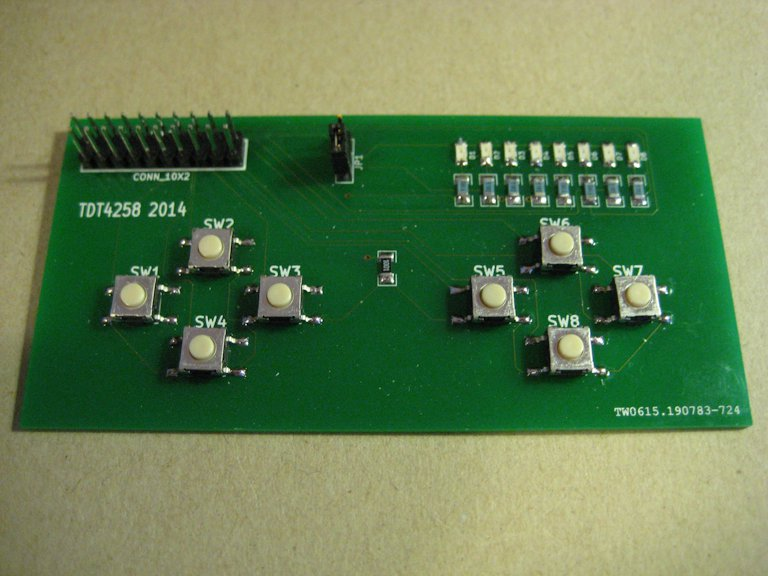
\includegraphics[width=0.5\textwidth]{images/gamepad.jpg}
  \caption{The prototype gamepad}\label{fig:gamepad}
\end{figure}




\subsection{Peripheral Reflex System}
The Peripheral Reflex System (PRS) is a network connecting the different peripheral modules together, allowing them to communicate directly without involving the CPU. The peripheral modules send each other \emph{reflex signals} routed by the PRS. On receiving such a signal, a peripheral module may perform some specific action depending on the signal received. By relieving the CPU of work, the PRS system can be used to improve energy efficiency. It is also suited for time-critical operations as it involves no variable-time software overhead.


\subsection{Low Energy Universal Asynchronous Receiver/Transmitter}\label{subsec:leuart}
TODO % TODO



\section{Energy Consumption}
TODO % Introduce this section

\subsection{Static and dynamic power}
The power used by a CMOS integrated circuit can be split into two main parts: \emph{dynamic power} and \emph{static power}. 

Dynamic power is the power needed to switch a circuit between two states. It depends on the clock frequency and activity level of a circuit, and is proportional to the square of the circuit voltage. In a clocked circuit it can be expressed as
$$P_{dynamic} = \alpha CV_{DD}^{2}f$$
where $\alpha$ is the activity level, $C$ is the capitance, $V_{DD}$ is the voltage, and $f$ is the clock frequency of the circuit.

Static power is power that dissipates due to leakage in the transistors of a circuit. It is linearly proportional to the circuit voltage, but independent of frequency. Static power can be expressed as
$$P_{static} = I_{leak}V_{DD}$$
where $I_{leak}$ is the current leaking through the transistors.

The total power used by the circuit is the sum of both dynamic and static power,
$$P_{total} = P_{dynamic} + P_{static}\ .$$
\cite{cmos-vlsi-design}


\subsection{Reducing energy consumption in the EFM32GG}
This section gives an overview of several ways to reduce the static and dynamic power consumption in the EFM32GG.

\subsubsection{Clock Gating}
Clock gating is a technique that reduces dynamic power consumption by disconnecting the clock from unused circuits. The EFM32GG uses automatic clock gating, and supports manual clock gating of both core modules and peripherals on an individual basis (see section \ref{sec:cmu}). Some energy can be saved by turning clocks on and off as the individual peripherals are needed.\cite{efm32-energy-optimization} 


\subsubsection{Disabling RAM blocks}
In the EFM32GG there is a static power dissipation in the RAM blocks of approximately 170 nA per 32 KB block. This constitutes a considerable amount when the device is in EM2 or EM3 energy modes. The RAM blocks can be disabled individually, and this is explained in section \ref{sec:emu}.\cite{efm32-energy-optimization}


\subsubsection{Increasing CPU frequency}
By increasing the clock frequency of the CPU it is possible to reduce its overall static power consumption. An increased frequency usually means that the CPU will finish its computations sooner, allowing it to stay in low energy modes for a larger fraction of the time. Increasing the frequency will also cause an increase in dynamic power consumption, but this is cancelled out by the similar reduction in processing time. There are some exceptional cases where the CPU processing speed is limited by wait-states in bus protocols. In such a case, the frequency should be increased within the imposed bounds.\cite{efm32-energy-optimization}


\subsubsection{Optimizing peripheral clocks}
The EFM32GG has several clocks and oscilliators running at different frequencies. By using a slower clock for the peripherals, the associated dynamic power consumption is reduced. It is optimal to selecting the slowest clock that satisfies the application requirements. Clock prescalers in the CMU or the individual peripherals can be used to adjust the frequency further. Clocks and oscilliators are controlled by the Clock Management Unit, described in section \ref{sec:cmu}.\cite{efm32-energy-optimization} 
% Relevant optimization techniques:
%  - Changing prescalers on-the-go to run at the fastest possible speed without introducing wait-states


\subsubsection{Reducing Bias Current of Analog Peripherals}
Most analog peripherals in the EFM32GG use something called a \emph{bias current}. It is possible to reduce this bias current to reduce power consumption, but this will affect the analog performance.\cite{efm32-energy-optimization}
% TODO(maybe): Expand this section by explaining what a bias current is


\subsubsection{Cache Optimization}
Several optimizations can be made by utilizing the caches of the EFM32GG. When a memory read or instruction fetch is satisfied from the cache, the processor avoids possible wait-states and memory reads and energy is saved. To optimize use of the 512 byte instruction cache of the EFM32GG, loops with a large number of instructions should be avoided. It is possible to measure cache misses and cache hits by reading performance counter registers.\cite{efm32-energy-optimization}
% TODO(optional): Write more about data caches in the EFM32GG. Should possibly be in a different section.


\subsubsection{Compiler optimizations}
As a rule of thumb, using a higher compiler optimization-level will result in more energy-efficient code.
% Relevant optimization techniques:
%  - optimizing for smaller program size vs speed


%--------------------------------------------------------------------
% Other optimization techniques that might be put into this section: 
% (from the Energy Optization Application Note)
%
%  - Use interrupts instead of busy wait
%  - Use wait-for-event instead of interrupts
%  - Use peripheral reflex system
%  - Saving power with DMA
%--------------------------------------------------------------------


\section{Direct Memory Access controller}
Direct Memory Access (DMA) is a technique in which I/O devices use the CPU bus to access the memory directly without involving the CPU. 
% TODO(maybe): Mention benefits of offloading work from the CPU
This is usually achieved by having a DMA controller, a specialized hardware component that can transfer data between memory and I/O devices, without direct interaction from the CPU. The I/O devices will be unaware that the transfer is being done by the DMA controller and not the CPU. An alternative to using a DMA controller for I/O is to do programmed input/output, where the CPU either uses interrupts or busy-wait to continually service an I/O device. DMA usually benefits over this approach as it allows the CPU to perform other work, or to enter low energy modes.
% TODO(maybe): Mention bus clogging and CPU idling. How can the DMA share a bus with the CPU?
It is possible to run the DMA in EM2 by using the LEUART module (see section \ref{subsec:leuart}).

\subsection{Configuration and use}
The DMA controller has 12 independent \emph{channels}. These can be triggered from either peripherals or software to start a DMA cycle. During a cycle, the DMA controller will read a \emph{channel descriptor} from system memory corresponding to that channel(?), and perform one or more DMA transfers as specified by the channel descriptor (and the DMA configuration?).

\subsubsection{Channel Configuration}
Before using a peripheral module together with the controller, a DMA channel must be configured to receive that peripheral's requests. This is done by writing to the channel control registers DMA\_CHx\_CTRL. These registers have two components: SOURCESEL, used to select which peripheral to listen to, and SIGSEL that specifies the signal to listen to of that peripheral.

\subsubsection{DMA Cycles}
A DMA cycle consists of several DMA transfers in which the controller transfers a single byte or word from one memory location to another. The controller might need several cycles in order to completely service a request. The behaviour of the controller during a cycle must be specified in the channel descriptor by setting a cycle type in the cycle\_ctrl bits.

\subsubsection{Channel Descriptors}
Channel descriptors are used to configure the behaviour of the DMA controller during a single DMA cycle. The channel descriptors must be stored in a contiguous area of memory called the \emph{channel control data structure}. The channel controll data structure itself consists of a primary and an alternate data structure, and these are lists of channel descriptors. It is the responsibility of the software to allocate the channel control data structures, and to write the channel descriptors needed. In addition, the base address of the channel control data structure needs to be written to the controller register DMA\_CTRLBASE. When reading the channel control data structure, the controller uses the lower eight bits to address channel descriptors. For this reason, the base address of the data structure must be at an address like 0xXXXXXX00.

A channel descriptor contains the following elements:
\begin{itemize}
	\item src\_data\_end\_ptr, a pointer to the ending address of the source data.
	\item dst\_data\_end\_ptr, a pointer to the ending address of the destination data.
	\item channel\_cfg, provides control information such as cycle type and R\_power.
\end{itemize}
At the start of a DMA cycle, the controller will read the channel\_cfg from memory. After completing the cycle, an updated channel\_cfg will be written back.


\section{Generating Sounds}
When interpreting a sound as a signal, we speak about properties of the sound such as frequency, period, and amplitude. Here frequency and period (the inverse frequency) describes the pitch of a sound, while amplitude describes the loudness. In a typical speaker, a voltage signal is converted directly into sound waves. Here the voltage signal is an accurate model of the sound wave and has the same frequency and amplitude. The range of sounds that can be perceived by a human being is from 20Hz to 20KHz.\cite{compendium}
% TODO: Write about how different tones can be generated
